\section{Autorisierung}

Wie bereits im Entity-relationship Diagramm \ref{fig:erd} gezeigt wurde, wird die Rolle eines Benutzers in Form eines \emph{ActiveRecord::Enum} abgebildet.
Darauf wird auch der Default-Wert \enquote{candidate} gesetzt, sodass neue Benutzer automatisch dieser Rolle zugeteilt werden.

\begin{codebox}
\begin{minted}{ruby}
class User < ApplicationRecord
  enum :role, { admin: 'admin', candidate: 'candidate' }, default: :candidate
end
\end{minted}
\end{codebox}

Die Benutzerrolle kann dann auf jeder User-Instanz folgendermassen abgerufen werden:

\begin{figure}[H]
  \centering
  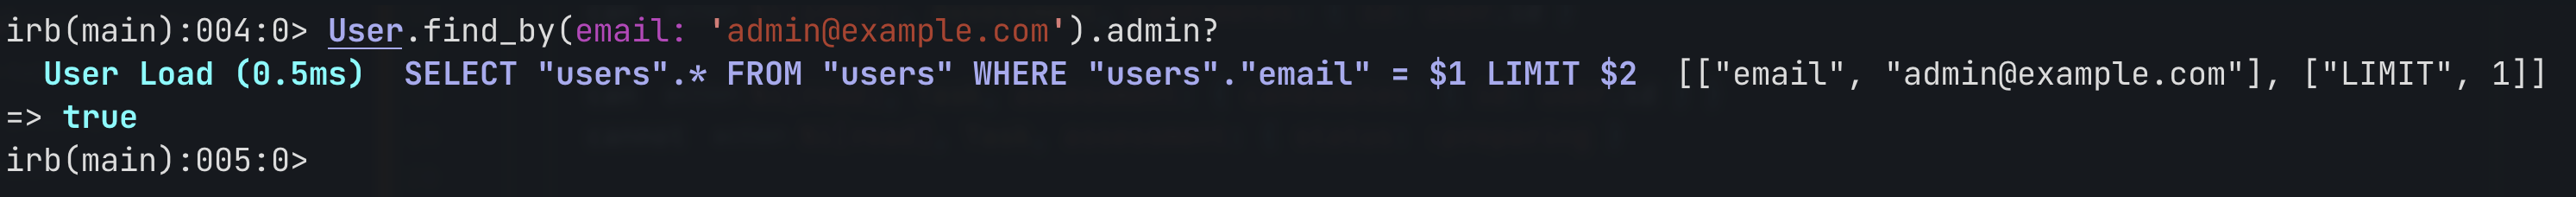
\includegraphics[width=\textwidth]{images/enum.png}
\end{figure}

Basierend auf der Benutzerrolle werden dann die 

\begin{codebox}
\begin{minted}{ruby}
def candidate_abilities(user)
  can %i[index], Assessment, candidates: { id: user.id }

  ...
end
\end{minted}
\end{codebox}

Ein Bewerber kann:
\begin{itemize}
  \item Nur die Assessments sehen, in denen dieser auch teilnimmt
  \item Tasks ansehen, allerdings erst, wenn das Assessment durch einen Admin gestartet wurde
  \item Lösungen erstellen und bearbeiten
\end{itemize}
